\chapter{Assignment: \protect\\ Hierarchical Clustering}
\label{hw:arheo_hierarchical_clustering}

\newthought{Shards belong to different time periods}. Periods are described with 22 numeric variables, each defining the likelihood of a shard belonging to the said period. First, let us visualize the data in a visualization that shows the value of numeric variables with color - the higher the value, the brighter the number. Such a visualization is called a \widget{Heat Map}.

\begin{figure}[h]
    \centering
    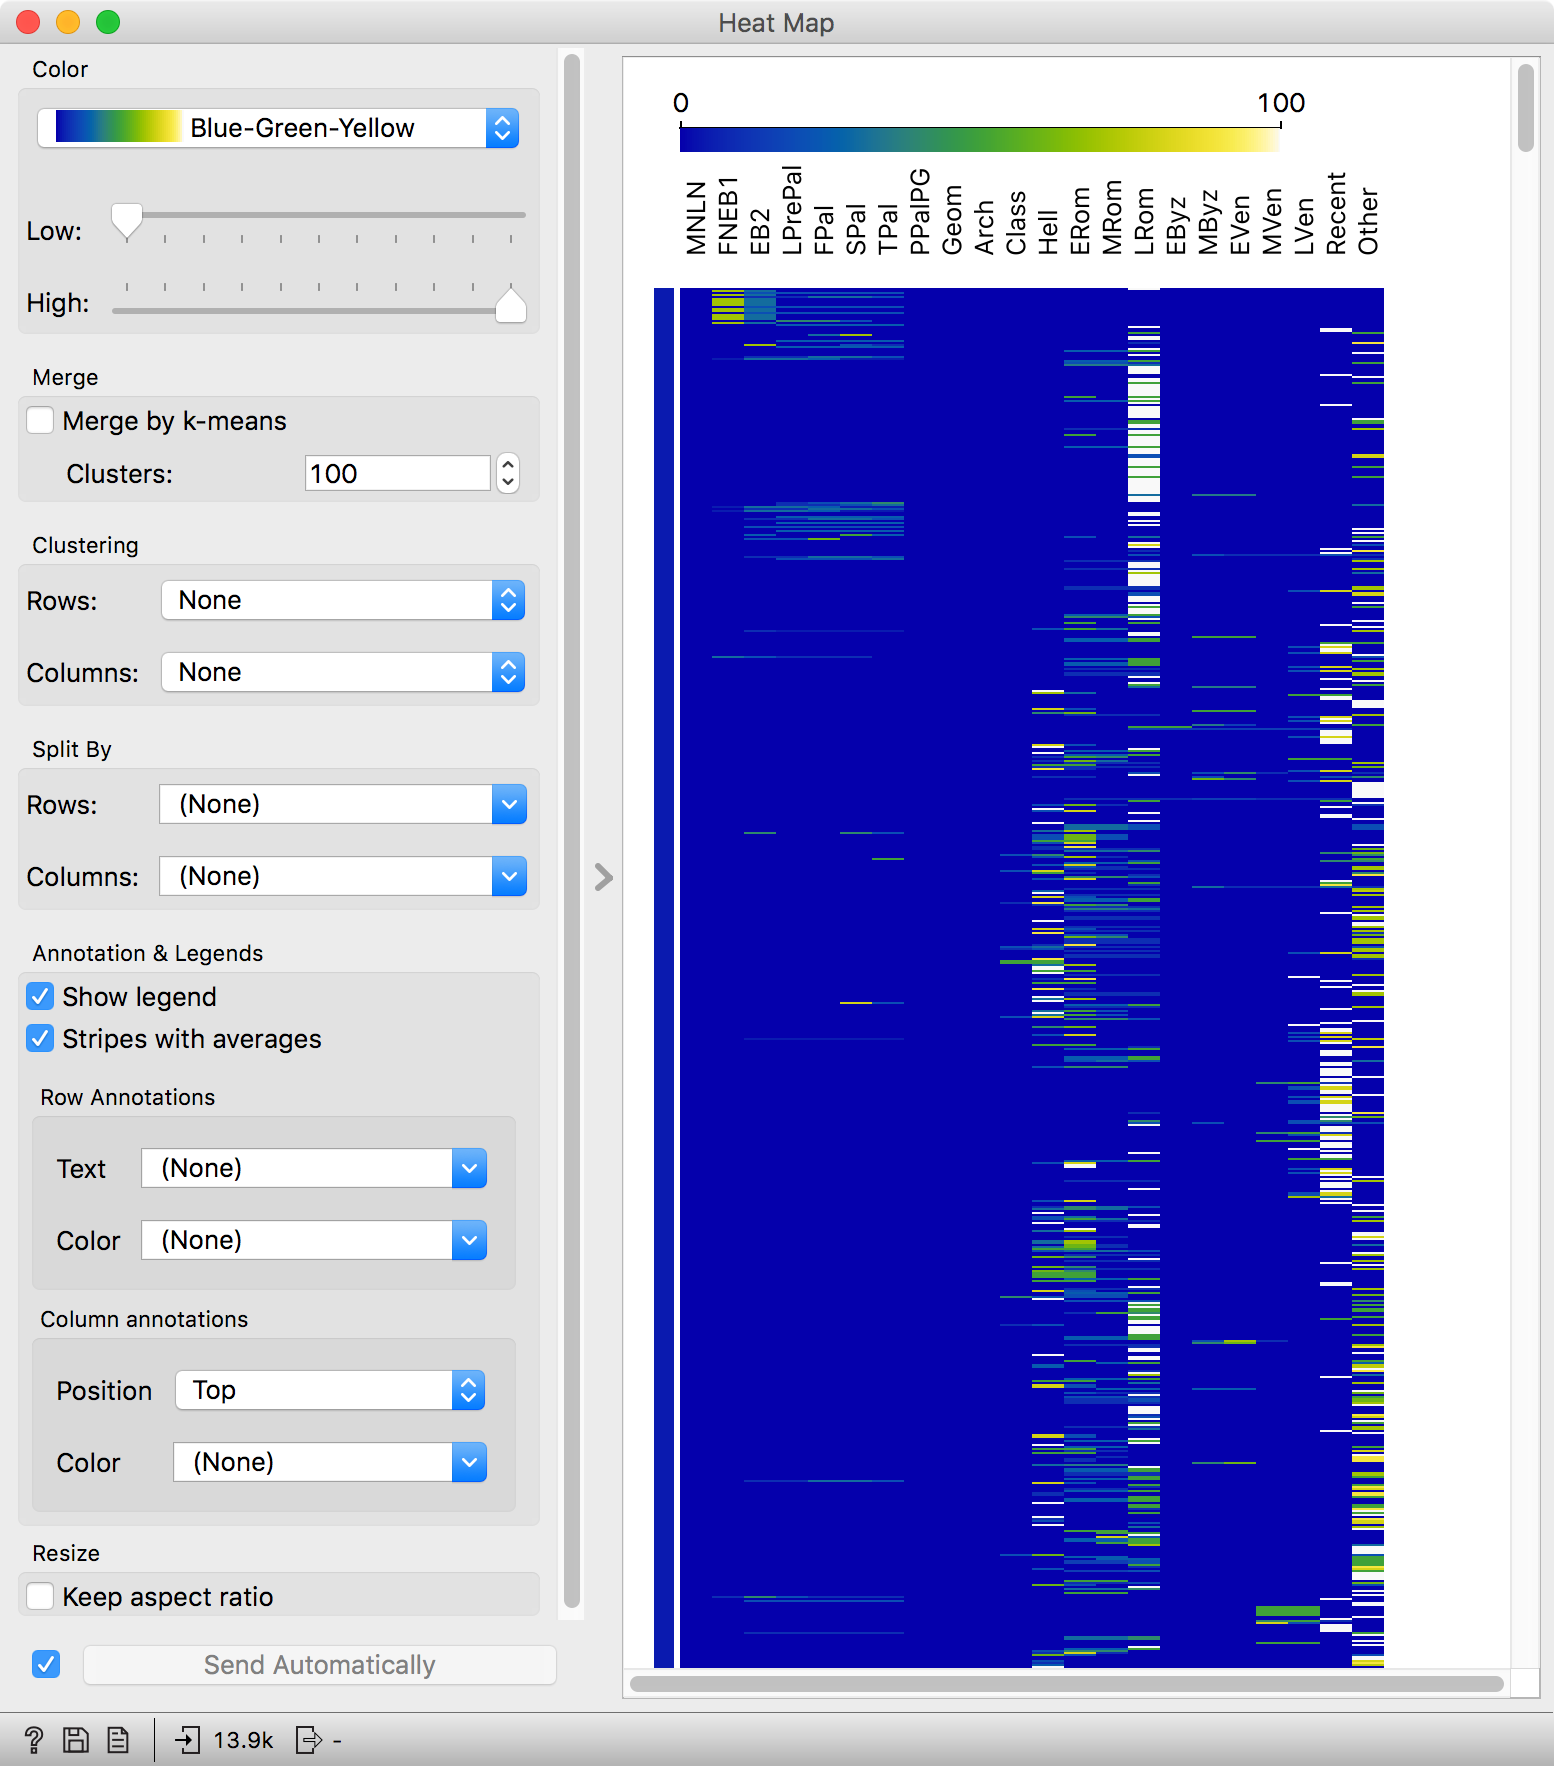
\includegraphics[scale=0.35]{heat-map-original.png}
    \caption{$\;$} % empty caption for proper page setting
\end{figure}

By default, Heat Map shows each data instance in a row and maps the values to the color scale. But our data is so unorganized, there is no way we can make sense of it! First, since we have many rows in our data set, let us join together rows that are the most similar. We will do this with \textit{Merge by k-means} option and set the number of clusters to 100. This is keep only 100 most different rows.

Visualization got simpler, but it is still unorganized. Would it be nice to have similar rows closer together? Of course it would! We can use hierarchical clustering to re-order rows, so that similar rows will be put next to each other. Use \textit{Clustering (opt. ordering)} - the plot now makes much more sense!

\begin{wrapfigure}{o}{1.05\textwidth}
    \vspace{-0.1cm}
    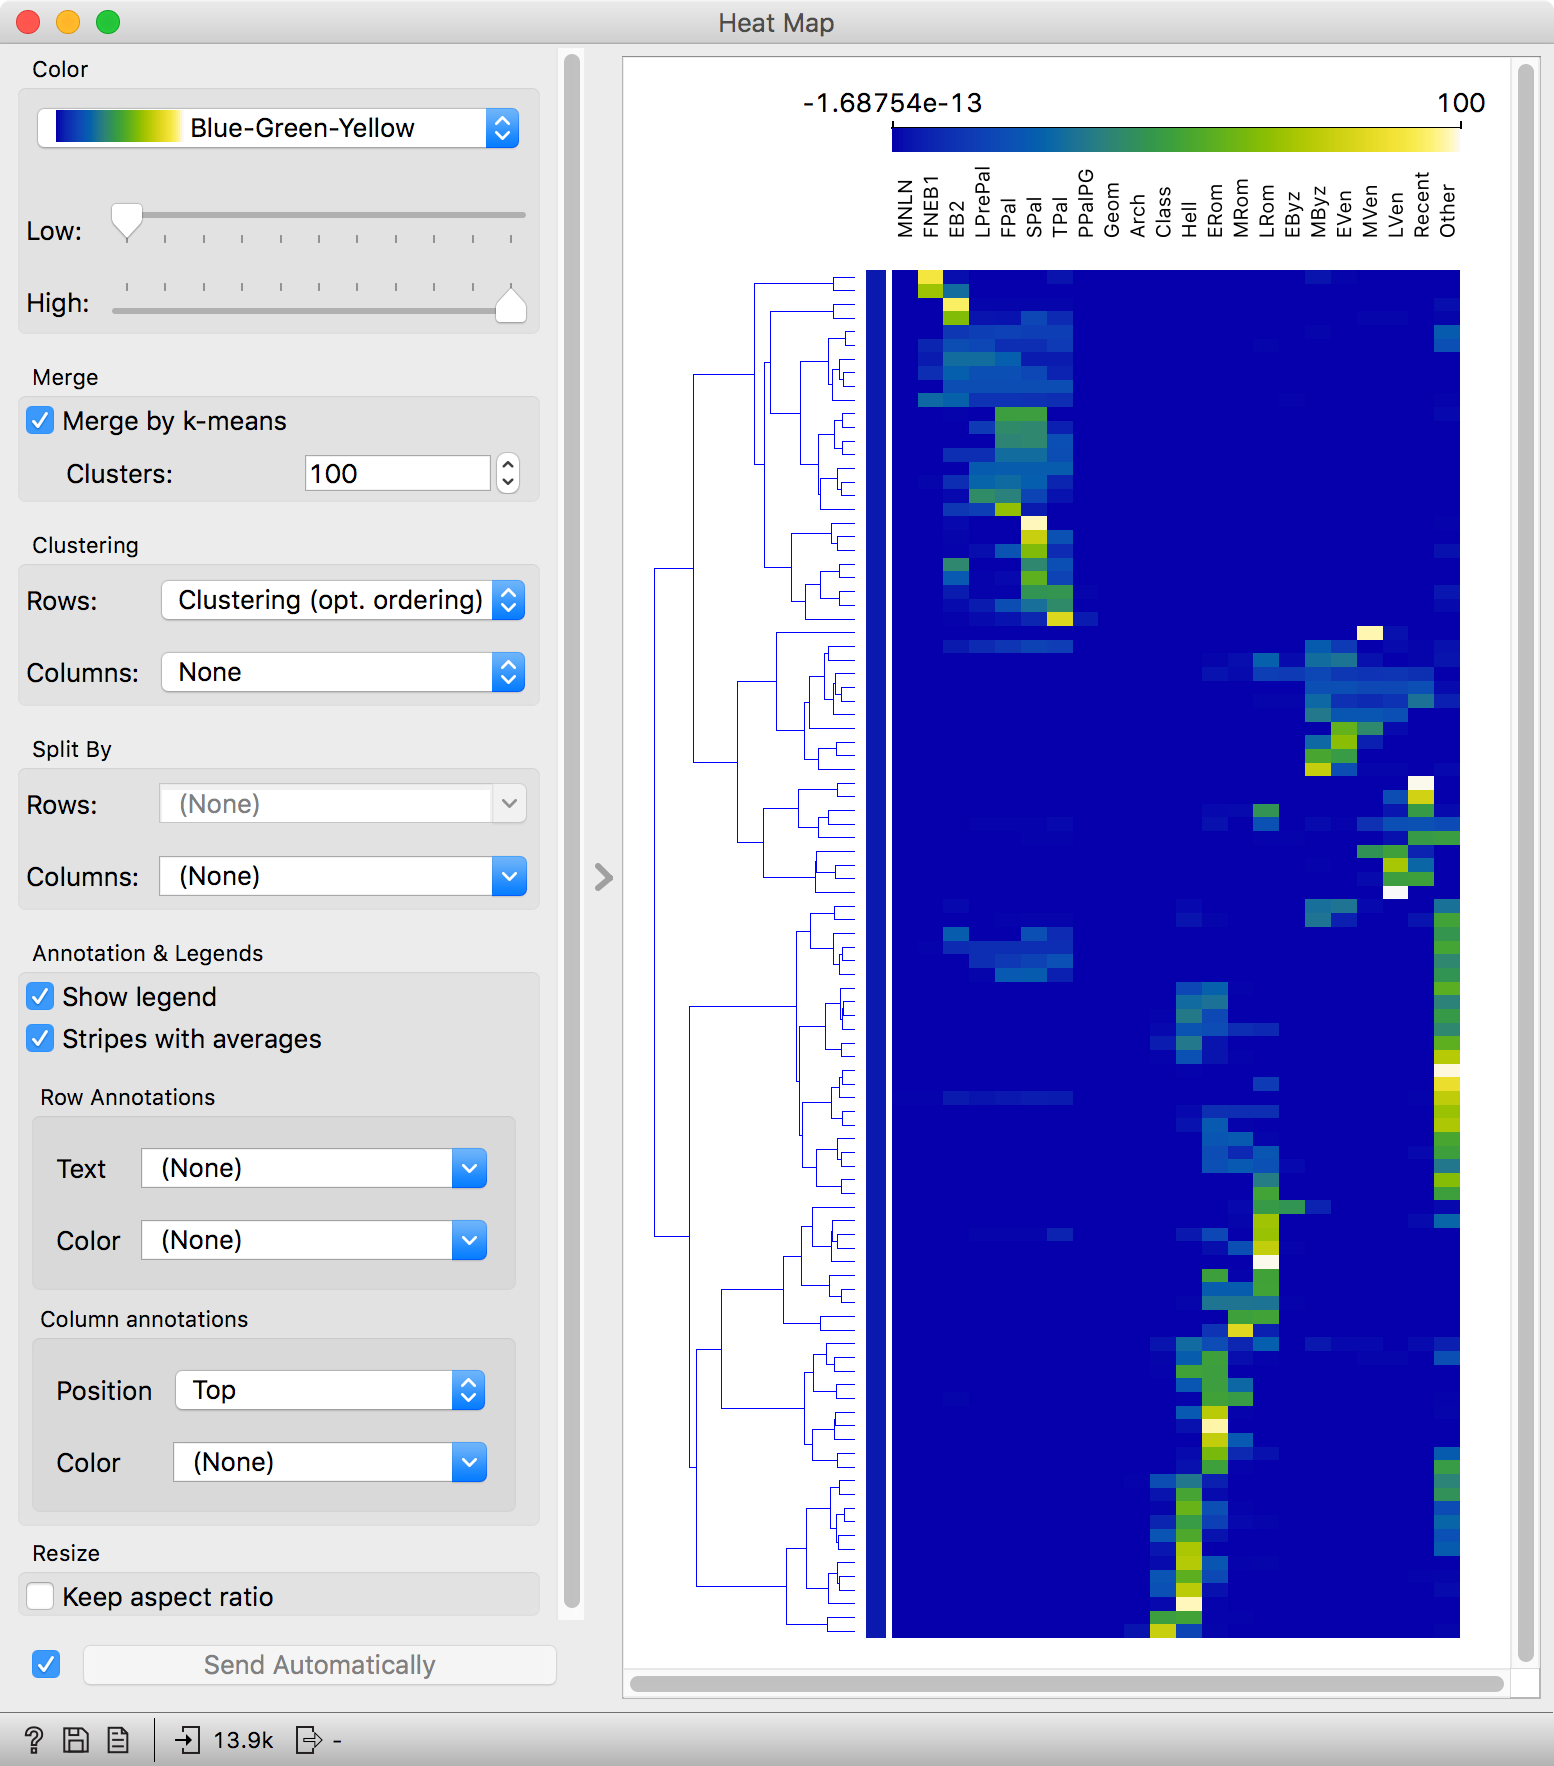
\includegraphics[scale=0.4]{heat-map-clustered.png}
\end{wrapfigure}

In the top left corner, we have shards from the early periods. In the bottom central part shards from Roman and Hellenic periods. And in the middle right part recent or unidentified shards.

We can repeat the same, but a more exact procedure, with \widget{Hierarchical Clustering}. First, let us pass the data to \widget{Distances} to compute the distance matrix. As our data has a fair number of dimensions (22 to be precise), we will use \textit{cosine distance} and \textit{Ward linkage} for the measure of cluster similarity.

In Hierarchial Clustering, we see a large dendrogram. To make it easier to read, set \textit{Max depth} to 10 (this will cut the tree at the tenth split). Use Zoom to zoom out as much as possible.

\begin{figure*}[h]
    \centering
    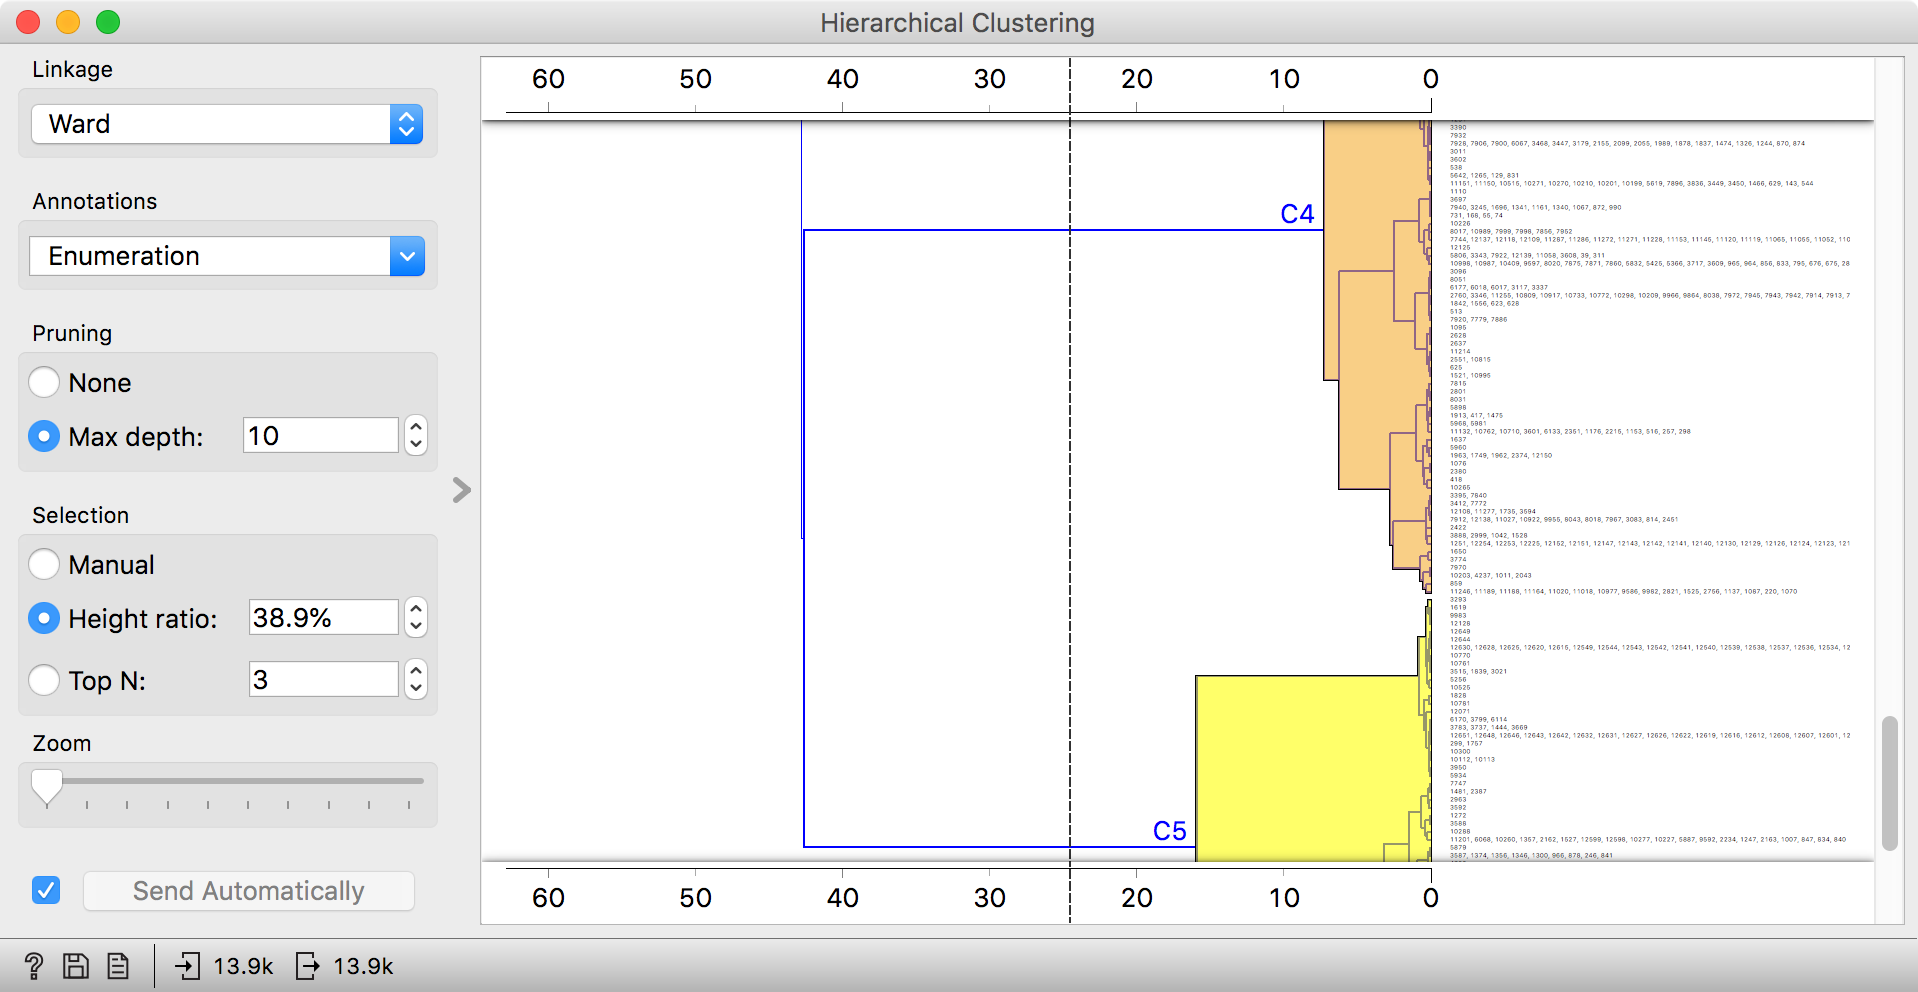
\includegraphics[scale=0.45]{hierarchical-clustering.png}
    \caption{$\;$} % empty caption for proper page setting
\end{figure*}

\newpage

\begin{figure}[h]
    \centering
    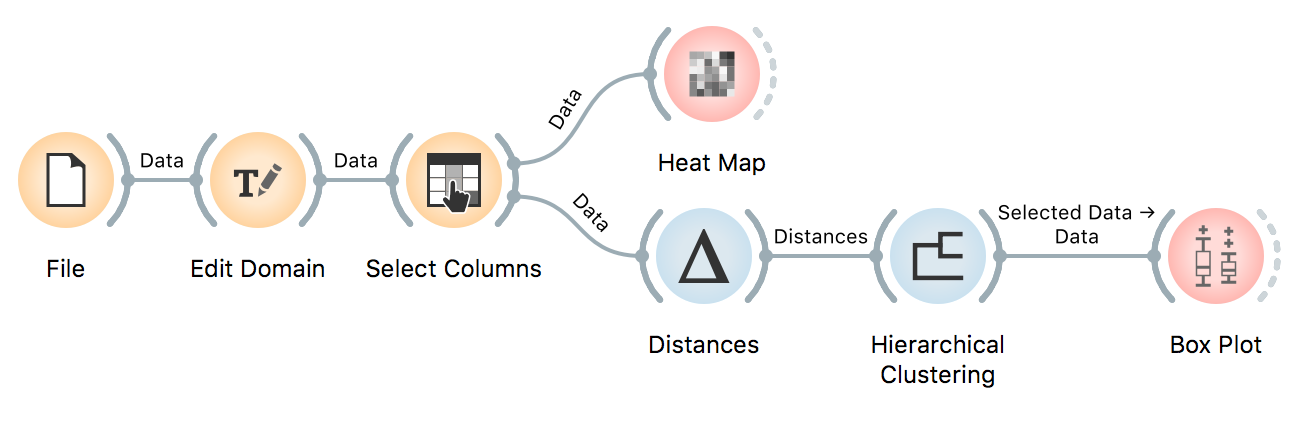
\includegraphics[scale=0.6]{workflow.png}
    \caption{$\;$} % empty caption for proper page setting
\end{figure}

\subsection{Assignment}

Use Box Plot to explore the clusters:
\begin{itemize}
    \item What is a good number of clusters? Why?
    \item Cut the dendrogram at the desired level (up to you). Which period(s) does each of the clusters represent? Could you name them?
    \item What defines each period? Use Box Plot with \textit{Data} output to find out.
\end{itemize}
